% !TEX root = BA-Bauer.tex
\subsection{Einstellungen}

\subsubsection{LCD-Kontrast \& LED-Helligkeit}
Das Gerät kann durch die zahlreichen Einsatzgebiete auch an vielen verschiedenen Orten eingesetzt werden. Um zu garantieren, dass die auf dem LCD-Display angezeigten Inhalte jederzeit erkennbar sind, soll der Benutzer die Möglichkeit haben den Kontrastwert des Displays einzustellen. Gleiches gilt für die Helligeit der LEDs. Soll das Gerät an einem unauffäligen Ort platziert werden, könnten aufblinkende LEDs störend wirken. Aus diesem Grund sind die Einstellungsfunktionen zum Einstellen des LCD-Kontrastes und LED-Helligkeit implementiert. In diesem Kapitel wird auf die Grundfunktionen beider Funktionen eingeganen. Beide Einstellungen basieren auf dem gleichen Prinzip, der PWM-Steuerung. 

\textbf{LCD-Kontrast}\\
In der Regel wird mithilfe eines einstellbaren Spannungsteilers (Potentiometer) eine Spannung an den $V0$-Pin des LCD-Moduls angelegt und damit der Kontrast geregelt. Diese Spannung kann auch mithilfe einer Pulsweitenmodulation erzeugt werden. Abbildung \ref{fig:lcdk25}, \ref{fig:lcdk50} und \ref{fig:lcdk75} zeigen die Auswirkungen der Änderung der Pulsweite auf den Kontrast des LCD-Displays. Für die Erzeugung des Pulsweitenmodulierten Signals wird Timer 1 des MCUs verwendet, welcher mit einer Frequenz von 10\,kHz Pulse erzeugt an einem Ausgangspin erzeugt, der mit dem $V0$-Pin des LCD-Moduls verbunden ist. Die Pulsweite wird durch das Beschreiben des $CCR$-Registers\footnote{Capture Compare Register} mit Werten von 0-100 eingestellt. In der Einstellungsfunktion entspricht der Wert des $CCR$-Registers dem Kontrastwert in \%.
\begin{figure}[h]
	\begin{minipage}{.3\linewidth}
		\centering
		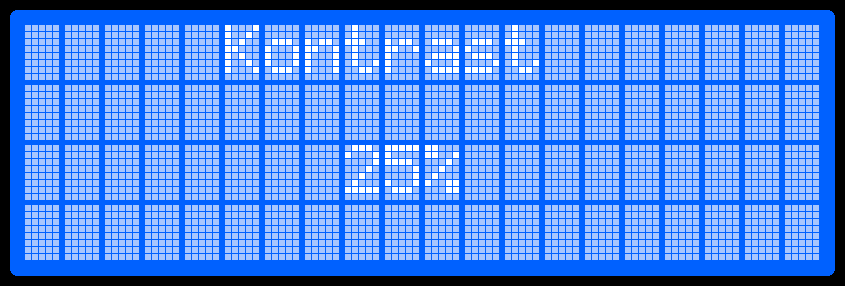
\includegraphics[width=\linewidth]{LCD-Screenshots/LCDKontrast25}
		\caption{LCD 25\% Kontrast}
		\label{fig:lcdk25}
	\end{minipage}
	\hfill
	\begin{minipage}{.3\linewidth}
		\centering
		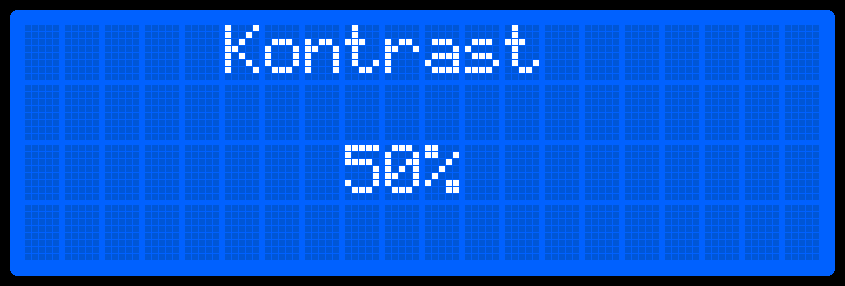
\includegraphics[width=\linewidth]{LCD-Screenshots/LCDKontrast50}
		\caption{LCD 50\% Kontrast}
		\label{fig:lcdk50}
	\end{minipage}
	\hfill
	\begin{minipage}{.3\linewidth}
		\centering
		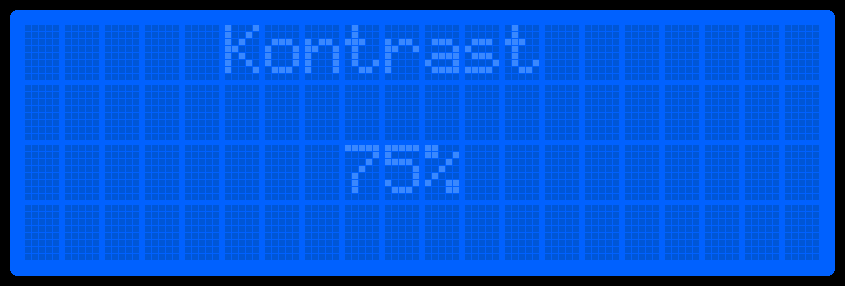
\includegraphics[width=\linewidth]{LCD-Screenshots/LCDKontrast75}
		\caption{LCD 75\% Kontrast}
		\label{fig:lcdk75}
	\end{minipage}
	\hfill
\end{figure}
Der Kontrastwert wird mithilfe des Encoders verändert und wird entsprechend auf dem Display angezeigt. Der Wert wird ehöht bei einer Drehbewegung in Uhrezigersinn und verringert bei einer Drehbewegung gegen den Uhrzeigersinn.

\textbf{LED-Helligkeit}\\
Wie auch der Kontrast des LCD-Displays, wird die Helligkeit der LEDs mithilfe eines Pulsweitenmodulierten Signals eingestellt. Für die LEDs wird Timer 9 des MCU mit einer Pulsfrequenz von 12,5\,kHz verwendet. Bei dieser Frequenz ist bei nierdrigen Helligkeiten kein Flackern der LEDs zu erkennen. Der Unterschied zu der LCD-Kontrast-Einstellungsfunktion ist lediglich das zu beschreibene Register und die angezeigte Überschrift auf dem LCD-Display.
\subsubsection{NPC ändern}
\subsubsection{Trigger}
\subsubsection{Aufnahme löschen}